%================================================
% PACKAGES AND THEMES
%================================================
\documentclass[t,aspectratio=169,xcolor=dvipsnames]{beamer}

\usetheme{SimplePlusAIC}

\usepackage{graphicx}
\usepackage{booktabs}
\usepackage{svg}
\usepackage{tcolorbox}
\usepackage{tikz}
\usepackage{makecell}

\newcommand*{\defeq}{\stackrel{\text{def}}{=}}
\usepackage{setspace}
\usepackage[T1]{fontenc}
\usepackage{helvet}
\usepackage{textgreek}
\usepackage{amsmath}
\usepackage{bm}
\usepackage{ragged2e}
\usepackage{xfrac}
\usepackage[loose]{units}
\usepackage{braket}
\usepackage{physics}
\usepackage{gensymb}
\usepackage{verbatim}
\usepackage{fancyvrb}

\usepackage[svgnames,table]{xcolor}
\arrayrulecolor{black}
\setlength{\arrayrulewidth}{0.20mm}
\renewcommand{\arraystretch}{1.35}

\newcommand{\tem}[1]{\textbf{\textcolor{red}{#1}}}

%================================================
% TITLE PAGE
%================================================
\title[CPU Scheduling]{CPU Scheduling}
\subtitle{Week 4: Contoh Soal dan Penyelesaian MLFQ}
\author[lectura.id/course/os]{lectura.id/course/os}
\institute[ITERA]{Program Studi Teknik Informatika \\ Institut Teknologi Sumatera}
\date{\textcolor{nyublue}{2026}}

%================================================
% BEGIN DOCUMENT
%================================================
\begin{document}

\begin{frame}
    \titlepage
\end{frame}

\begin{frame}
    \frametitle{OUTLINE}
    \framesubtitle{Peta materi pertemuan ini}
    \small
    \begin{spacing}{1.15}
        \tableofcontents
    \end{spacing}
\end{frame}

\begin{frame}
    \frametitle{Capaian Pembelajaran}
    \framesubtitle{Kemampuan yang ditargetkan setelah kuliah}
    \small
    \begin{enumerate}
        \item Mengingat kembali aturan dasar Multi-Level Feedback Queue (MLFQ).
        \item Memahami cara kerja MLFQ melalui simulasi contoh soal.
        \item Mampu menelusuri (tracing) eksekusi proses langkah demi langkah.
        \item Memahami bagaimana prioritas proses berubah seiring waktu.
    \end{enumerate}
    \begin{exampleblock}{Target Akhir}
        Setelah pertemuan ini, mahasiswa tidak hanya tahu teori MLFQ, tetapi \tem{bisa menyelesaikan} soal penjadwalan MLFQ dengan benar dan sistematis.
    \end{exampleblock}
\end{frame}

%================================================
% PART 1: REVIEW ATURAN MLFQ
%================================================
\section{Review Aturan MLFQ}

\begin{frame}
    \frametitle{Mengingat Kembali MLFQ}
    \framesubtitle{5 Aturan Emas MLFQ}
    \small
    Sebelum masuk ke contoh soal, mari kita ingat kembali aturan main MLFQ dengan bahasa yang sederhana:
    \vspace{0.3cm}
    \begin{enumerate}
        \item \textbf{Aturan 1:} Jika Prioritas A > Prioritas B, maka A berjalan (B menunggu).
        \item \textbf{Aturan 2:} Jika Prioritas A = Prioritas B, A dan B berjalan bergantian (Round-Robin).
        \item \textbf{Aturan 3:} Pekerjaan \tem{baru} selalu masuk ke antrean paling atas (prioritas tertinggi).
        \item \textbf{Aturan 4:} Jika pekerjaan menghabiskan jatah waktunya di suatu antrean, ia akan \tem{"turun kelas"} ke antrean di bawahnya.
        \item \textbf{Aturan 5 (Boost):} Setelah periode waktu tertentu ($S$), \tem{semua} pekerjaan dikembalikan ke antrean paling atas agar tidak ada yang kelaparan (starvation).
    \end{enumerate}
\end{frame}

\begin{frame}
    \frametitle{Apakah Aturan MLFQ Selalu Sama?}
    \framesubtitle{Variasi Implementasi di Dunia Nyata}
    \small
    \textbf{Tidak selalu!} Konsep dasarnya sama, tetapi \tem{parameter dan detail aturannya} bisa berbeda-beda tergantung sistem operasi (Windows, Solaris, dll).
    \vspace{0.3cm}
    \begin{itemize}
        \item \textbf{Jumlah Antrean:} Bisa 3, 4, atau bahkan 60 tingkat antrean.
        \item \textbf{Jatah Waktu (Time Quantum):} Biasanya semakin rendah prioritasnya, jatah waktunya semakin \tem{panjang} (contoh: Q3=10ms, Q2=20ms, Q1=40ms).
        \item \textbf{Interval Boost ($S$):} Kapan semua pekerjaan diangkat kembali ke atas? Jika terlalu cepat, pekerjaan interaktif terganggu. Jika terlalu lambat, terjadi \textit{starvation}.
        \item \textbf{Aturan I/O (Accounting):} Di MLFQ modern, sistem \tem{mengingat} total waktu CPU yang dipakai di suatu tingkat, meskipun pekerjaan tersebut sering berhenti untuk I/O (mencegah \textit{gaming the system}).
    \end{itemize}
\end{frame}

%================================================
% PART 2: CONTOH SOAL 1 (DASAR)
%================================================
\section{Contoh Soal 1 (Dasar)}

\begin{frame}
    \frametitle{Skenario Sistem (Soal 1)}
    \framesubtitle{Spesifikasi Antrean MLFQ}
    \small
    Bayangkan kita memiliki sistem MLFQ dengan \textbf{3 tingkat antrean}:
    \vspace{0.3cm}
    \begin{itemize}
        \item \textbf{Q3 (Prioritas Tertinggi):} Jatah waktu (Time Quantum) = \tem{10 ms}
        \item \textbf{Q2 (Prioritas Menengah):} Jatah waktu (Time Quantum) = \tem{20 ms}
        \item \textbf{Q1 (Prioritas Terendah):} Jatah waktu (Time Quantum) = \tem{40 ms}
    \end{itemize}
    \vspace{0.3cm}
    \begin{alertblock}{Aturan Tambahan}
        Setiap \tem{50 ms}, sistem melakukan \textbf{Priority Boost} (Aturan 5). Semua pekerjaan yang belum selesai akan diangkat kembali ke Q3.
    \end{alertblock}
\end{frame}

\begin{frame}
    \frametitle{Daftar Pekerjaan (Jobs)}
    \framesubtitle{Siapa saja yang akan dieksekusi?}
    \small
    Terdapat 3 pekerjaan yang datang ke sistem kita:
    \vspace{0.3cm}
    \begin{table}[]
        \centering
        \begin{tabular}{lcc}
            \toprule
            \textbf{Nama Job} & \textbf{Waktu Datang (Arrival)} & \textbf{Kebutuhan CPU (Burst)} \\
            \midrule
            \textbf{Job A} & 0 ms & 45 ms \\
            \textbf{Job B} & 15 ms & 15 ms \\
            \textbf{Job C} & 22 ms & 5 ms \\
            \bottomrule
        \end{tabular}
    \end{table}
    \vspace{0.3cm}
    Mari kita simulasikan perjalanannya \tem{langkah demi langkah}!
\end{frame}

%================================================
% PART 3: PENYELESAIAN SOAL 1
%================================================
\section{Penyelesaian Soal 1}

\begin{frame}
    \frametitle{Langkah 1: Waktu = 0 ms}
    \framesubtitle{Kedatangan Job A}
    \small
    \begin{itemize}
        \item \textbf{Kejadian:} Job A datang.
        \item \textbf{Aksi:} Sesuai Aturan 3, Job A masuk ke antrean paling atas (Q3).
        \item \textbf{Status Antrean:}
        \begin{itemize}
            \item Q3: [ \tem{A} ]
            \item Q2: [ ]
            \item Q1: [ ]
        \end{itemize}
        \item \textbf{Eksekusi:} CPU mulai menjalankan Job A. Jatah waktu Q3 adalah 10 ms.
    \end{itemize}
    \vspace{0.3cm}
    \begin{exampleblock}{Catatan}
        Sisa waktu Job A = 45 ms.
    \end{exampleblock}
\end{frame}

\begin{frame}
    \frametitle{Langkah 2: Waktu = 10 ms}
    \framesubtitle{Job A Turun Kelas}
    \small
    \begin{itemize}
        \item \textbf{Kejadian:} Job A sudah berjalan selama 10 ms.
        \item \textbf{Aksi:} Job A menghabiskan jatah waktu Q3 (10 ms). Sesuai Aturan 4, Job A \tem{"turun kelas"} ke Q2.
        \item \textbf{Status Antrean:}
        \begin{itemize}
            \item Q3: [ ]
            \item Q2: [ \tem{A} ]
            \item Q1: [ ]
        \end{itemize}
        \item \textbf{Eksekusi:} Karena Q3 kosong, CPU lanjut menjalankan Q2. Job A kembali berjalan. Jatah waktu Q2 adalah 20 ms.
    \end{itemize}
    \vspace{0.3cm}
    \begin{exampleblock}{Catatan}
        Sisa waktu Job A = 45 - 10 = \textbf{35 ms}.
    \end{exampleblock}
\end{frame}

\begin{frame}
    \frametitle{Langkah 3: Waktu = 15 ms}
    \framesubtitle{Kedatangan Job B (Interupsi!)}
    \small
    \begin{itemize}
        \item \textbf{Kejadian:} Job B datang!
        \item \textbf{Aksi:} Job B masuk ke Q3. Saat ini Job A sedang berjalan di Q2 (baru jalan 5 ms). Karena ada pekerjaan di Q3, CPU \tem{menghentikan} Job A sementara (Aturan 1).
        \item \textbf{Status Antrean:}
        \begin{itemize}
            \item Q3: [ \tem{B} ]
            \item Q2: [ \tem{A} ] (A baru pakai 5 ms dari jatah 20 ms-nya)
            \item Q1: [ ]
        \end{itemize}
        \item \textbf{Eksekusi:} CPU menjalankan Job B dari Q3.
    \end{itemize}
    \vspace{0.3cm}
    \begin{exampleblock}{Catatan}
        Sisa waktu Job A = 35 - 5 = \textbf{30 ms}. Sisa jatah A di Q2 = \textbf{15 ms}.\\
        Sisa waktu Job B = \textbf{15 ms}.
    \end{exampleblock}
\end{frame}

\begin{frame}
    \frametitle{Langkah 4: Waktu = 22 ms}
    \framesubtitle{Kedatangan Job C}
    \small
    \begin{itemize}
        \item \textbf{Kejadian:} Job C datang!
        \item \textbf{Aksi:} Job C masuk ke Q3. Saat ini Job B sedang berjalan di Q3 (sudah jalan 7 ms). Job C antre di belakang Job B.
        \item \textbf{Status Antrean:}
        \begin{itemize}
            \item Q3: [ \tem{B}, \tem{C} ] (B sedang jalan)
            \item Q2: [ \tem{A} ]
            \item Q1: [ ]
        \end{itemize}
        \item \textbf{Eksekusi:} CPU lanjut menjalankan Job B sampai jatah waktu Q3-nya (10 ms) habis.
    \end{itemize}
    \vspace{0.3cm}
    \begin{exampleblock}{Catatan}
        Sisa waktu Job C = \textbf{5 ms}.
    \end{exampleblock}
\end{frame}

\begin{frame}
    \frametitle{Langkah 5: Waktu = 25 ms}
    \framesubtitle{Job B Turun Kelas}
    \small
    \begin{itemize}
        \item \textbf{Kejadian:} Job B sudah berjalan 10 ms (dari waktu 15 ke 25).
        \item \textbf{Aksi:} Job B menghabiskan jatah waktu Q3. Job B \tem{"turun kelas"} ke Q2, antre di belakang A.
        \item \textbf{Status Antrean:}
        \begin{itemize}
            \item Q3: [ \tem{C} ]
            \item Q2: [ \tem{A}, \tem{B} ]
            \item Q1: [ ]
        \end{itemize}
        \item \textbf{Eksekusi:} CPU melihat Q3 ada isinya (Job C). CPU mulai menjalankan Job C.
    \end{itemize}
    \vspace{0.3cm}
    \begin{exampleblock}{Catatan}
        Sisa waktu Job B = 15 - 10 = \textbf{5 ms}.
    \end{exampleblock}
\end{frame}

\begin{frame}
    \frametitle{Langkah 6: Waktu = 30 ms}
    \framesubtitle{Job C Selesai!}
    \small
    \begin{itemize}
        \item \textbf{Kejadian:} Job C berjalan selama 5 ms (dari 25 ke 30).
        \item \textbf{Aksi:} Kebutuhan Job C hanya 5 ms. Jadi, Job C \tem{SELESAI} dan keluar dari sistem!
        \item \textbf{Status Antrean:}
        \begin{itemize}
            \item Q3: [ ]
            \item Q2: [ \tem{A}, \tem{B} ]
            \item Q1: [ ]
        \end{itemize}
        \item \textbf{Eksekusi:} Q3 kosong. CPU turun ke Q2. Di Q2 ada A dan B. Giliran Job A yang jalan (karena A masuk Q2 lebih dulu).
    \end{itemize}
    \vspace{0.3cm}
    \begin{exampleblock}{Catatan}
        Job C selesai pada waktu \textbf{30 ms}.
    \end{exampleblock}
\end{frame}

\begin{frame}
    \frametitle{Langkah 7: Waktu = 45 ms}
    \framesubtitle{Job A Turun Kelas (Lagi)}
    \small
    \begin{itemize}
        \item \textbf{Kejadian:} Job A melanjutkan sisa jatah waktunya di Q2 (15 ms). Ia berjalan dari waktu 30 ke 45.
        \item \textbf{Aksi:} Job A menghabiskan total jatah waktu Q2 (20 ms). Job A \tem{"turun kelas"} ke Q1.
        \item \textbf{Status Antrean:}
        \begin{itemize}
            \item Q3: [ ]
            \item Q2: [ \tem{B} ]
            \item Q1: [ \tem{A} ]
        \end{itemize}
        \item \textbf{Eksekusi:} Q3 kosong, Q2 ada isinya. CPU menjalankan Job B di Q2.
    \end{itemize}
    \vspace{0.3cm}
    \begin{exampleblock}{Catatan}
        Sisa waktu Job A = 30 - 15 = \textbf{15 ms}.
    \end{exampleblock}
\end{frame}

\begin{frame}
    \frametitle{Langkah 8: Waktu = 50 ms}
    \framesubtitle{Job B Selesai \& PRIORITY BOOST!}
    \small
    \begin{itemize}
        \item \textbf{Kejadian 1:} Job B berjalan 5 ms (dari 45 ke 50). Sisa waktu B habis. Job B \tem{SELESAI}!
        \item \textbf{Kejadian 2:} Waktu menunjukkan \textbf{50 ms}. Waktunya \tem{Priority Boost} (Aturan 5)!
        \item \textbf{Aksi:} Semua pekerjaan yang tersisa (hanya Job A) diangkat kembali ke Q3.
        \item \textbf{Status Antrean:}
        \begin{itemize}
            \item Q3: [ \tem{A} ] (Naik dari Q1)
            \item Q2: [ ]
            \item Q1: [ ]
        \end{itemize}
        \item \textbf{Eksekusi:} CPU menjalankan Job A di Q3.
    \end{itemize}
    \vspace{0.3cm}
    \begin{exampleblock}{Catatan}
        Job B selesai pada waktu \textbf{50 ms}. Sisa waktu Job A = \textbf{15 ms}.
    \end{exampleblock}
\end{frame}

\begin{frame}
    \frametitle{Langkah 9: Waktu = 60 ms}
    \framesubtitle{Job A Turun Kelas (Setelah Boost)}
    \small
    \begin{itemize}
        \item \textbf{Kejadian:} Job A berjalan 10 ms di Q3 (dari 50 ke 60).
        \item \textbf{Aksi:} Job A menghabiskan jatah waktu Q3. Job A \tem{"turun kelas"} ke Q2.
        \item \textbf{Status Antrean:}
        \begin{itemize}
            \item Q3: [ ]
            \item Q2: [ \tem{A} ]
            \item Q1: [ ]
        \end{itemize}
        \item \textbf{Eksekusi:} CPU lanjut menjalankan Job A di Q2.
    \end{itemize}
    \vspace{0.3cm}
    \begin{exampleblock}{Catatan}
        Sisa waktu Job A = 15 - 10 = \textbf{5 ms}.
    \end{exampleblock}
\end{frame}

\begin{frame}
    \frametitle{Langkah 10: Waktu = 65 ms}
    \framesubtitle{Semua Selesai!}
    \small
    \begin{itemize}
        \item \textbf{Kejadian:} Job A berjalan 5 ms lagi (dari 60 ke 65).
        \item \textbf{Aksi:} Sisa waktu Job A habis. Job A \tem{SELESAI}!
        \item \textbf{Status Antrean:}
        \begin{itemize}
            \item Q3: [ ]
            \item Q2: [ ]
            \item Q1: [ ]
        \end{itemize}
        \item \textbf{Eksekusi:} Sistem kosong. CPU menganggur (idle).
    \end{itemize}
    \vspace{0.3cm}
    \begin{exampleblock}{Catatan}
        Job A selesai pada waktu \textbf{65 ms}. Simulasi berakhir!
    \end{exampleblock}
\end{frame}

%================================================
% PART 4: CONTOH SOAL 2 (LANJUT)
%================================================
\section{Contoh Soal 2 (Lanjut)}

\begin{frame}
    \frametitle{Skenario Sistem (Soal 2)}
    \framesubtitle{Tantangan Lebih Berat: 5 Pekerjaan}
    \small
    Aturan sistem masih sama:
    \begin{itemize}
        \item \textbf{Q3:} Jatah waktu = \tem{10 ms}
        \item \textbf{Q2:} Jatah waktu = \tem{20 ms}
        \item \textbf{Q1:} Jatah waktu = \tem{40 ms}
        \item \textbf{Priority Boost:} Setiap \tem{50 ms}
    \end{itemize}
    \vspace{0.3cm}
    \begin{table}[]
        \centering
        \begin{tabular}{lcc}
            \toprule
            \textbf{Nama Job} & \textbf{Waktu Datang (Arrival)} & \textbf{Kebutuhan CPU (Burst)} \\
            \midrule
            \textbf{Job A} & 0 ms & 30 ms \\
            \textbf{Job B} & 15 ms & 20 ms \\
            \textbf{Job C} & 25 ms & 15 ms \\
            \textbf{Job D} & 35 ms & 5 ms \\
            \textbf{Job E} & 42 ms & 10 ms \\
            \bottomrule
        \end{tabular}
    \end{table}
\end{frame}

%================================================
% PART 5: PENYELESAIAN SOAL 2
%================================================
\section{Penyelesaian Soal 2}

\begin{frame}
    \frametitle{Langkah 1: Waktu 0 - 15 ms}
    \framesubtitle{Awal Mula}
    \small
    \begin{itemize}
        \item \textbf{0 ms:} Job A datang ke Q3. CPU menjalankan A.
        \item \textbf{10 ms:} Job A menghabiskan jatah Q3 (10 ms). A \tem{turun kelas} ke Q2. CPU lanjut menjalankan A di Q2.
        \item \textbf{15 ms:} Job B datang ke Q3! Karena Q3 lebih tinggi dari Q2, Job B \tem{menginterupsi} Job A.
    \end{itemize}
    \vspace{0.3cm}
    \begin{exampleblock}{Status di 15 ms}
        Q3: [ \tem{B} ] (sedang jalan) \\
        Q2: [ \tem{A} ] (A sudah jalan 10ms di Q3 + 5ms di Q2. Sisa burst A = 15ms) \\
        Q1: [ ]
    \end{exampleblock}
\end{frame}

\begin{frame}
    \frametitle{Langkah 2: Waktu 15 - 35 ms}
    \framesubtitle{Kedatangan Beruntun}
    \footnotesize
    \begin{itemize}
        \item \textbf{25 ms:} Job B menghabiskan jatah Q3 (10 ms). B \tem{turun kelas} ke Q2. Bersamaan dengan itu, \textbf{Job C datang} ke Q3! CPU menjalankan C.
        \item \textbf{35 ms:} Job C menghabiskan jatah Q3 (10 ms). C \tem{turun kelas} ke Q2. Bersamaan dengan itu, \textbf{Job D datang} ke Q3! CPU menjalankan D.
    \end{itemize}
    \vspace{0.3cm}
    \begin{exampleblock}{Status di 35 ms}
        Q3: [ \tem{D} ] (sedang jalan) \\
        Q2: [ \tem{A}, \tem{B}, \tem{C} ] (Antre sesuai urutan masuk Q2) \\
        Q1: [ ]
    \end{exampleblock}
\end{frame}

\begin{frame}
    \frametitle{Langkah 3: Waktu 35 - 42 ms}
    \framesubtitle{Pekerjaan Pendek Selesai}
    \footnotesize
    \begin{itemize}
        \item \textbf{40 ms:} Job D hanya butuh 5 ms. Job D \tem{SELESAI}! Q3 kosong. CPU turun ke Q2 dan melanjutkan Job A (karena A paling depan di Q2).
        \item \textbf{42 ms:} Job E datang ke Q3! Job E \tem{menginterupsi} Job A lagi.
    \end{itemize}
    \vspace{0.3cm}
    \begin{exampleblock}{Status di 42 ms}
        Q3: [ \tem{E} ] (sedang jalan) \\
        Q2: [ \tem{A}, \tem{B}, \tem{C} ] (A baru jalan 2ms lagi di Q2. Total A jalan = 17ms. Sisa burst A = 13ms) \\
        Q1: [ ]
    \end{exampleblock}
\end{frame}

\begin{frame}
    \frametitle{Langkah 4: Waktu 50 ms}
    \framesubtitle{PRIORITY BOOST!}
    \footnotesize
    \begin{itemize}
        \item \textbf{50 ms:} Waktunya \tem{Priority Boost}! Semua pekerjaan yang ada di Q2 dan Q1 diangkat kembali ke Q3.
        \item Saat ini Job E sedang berjalan (sudah jalan 8 ms, sisa 2 ms). Job A, B, dan C naik ke Q3 di belakang E.
    \end{itemize}
    \vspace{0.3cm}
    \begin{exampleblock}{Status di 50 ms}
        Q3: [ \tem{E}, \tem{A}, \tem{B}, \tem{C} ] (E lanjut jalan) \\
        Q2: [ ] \\
        Q1: [ ]
    \end{exampleblock}
\end{frame}

\begin{frame}
    \frametitle{Langkah 5: Waktu 50 - 80 ms}
    \framesubtitle{Penyelesaian Akhir}
    \small
    \begin{itemize}
        \item \textbf{52 ms:} Job E selesai (butuh 2 ms lagi). CPU lanjut ke Job A.
        \item \textbf{62 ms:} Job A menghabiskan jatah Q3 (10 ms). A turun ke Q2. CPU lanjut ke Job B. (Sisa burst A = 3ms).
        \item \textbf{72 ms:} Job B menghabiskan jatah Q3 (10 ms). Karena sisa burst B memang 10 ms, Job B \tem{SELESAI}! CPU lanjut ke Job C.
        \item \textbf{77 ms:} Job C selesai (sisa burst C hanya 5 ms). Q3 kosong.
        \item \textbf{80 ms:} CPU turun ke Q2, menjalankan sisa Job A (3 ms). Job A \tem{SELESAI}!
    \end{itemize}
\end{frame}

\begin{frame}
    \frametitle{Ringkasan Waktu Penyelesaian (Soal 2)}
    \framesubtitle{Kapan setiap pekerjaan selesai?}
    \footnotesize
    \begin{table}[]
        \centering
        \begin{tabular}{lccc}
            \toprule
            \textbf{Nama Job} & \textbf{Waktu Datang} & \textbf{Burst Time} & \textbf{Waktu Selesai} \\
            \midrule
            \textbf{Job D} & 35 ms & 5 ms & \tem{40 ms} \\
            \textbf{Job E} & 42 ms & 10 ms & \tem{52 ms} \\
            \textbf{Job B} & 15 ms & 20 ms & \tem{72 ms} \\
            \textbf{Job C} & 25 ms & 15 ms & \tem{77 ms} \\
            \textbf{Job A} & 0 ms & 30 ms & \tem{80 ms} \\
            \bottomrule
        \end{tabular}
    \end{table}
    \vspace{0.1cm}
    \begin{alertblock}{Pelajaran Penting}
        Meskipun Job A datang pertama, ia selesai paling akhir karena butuh waktu lama. Job D dan E yang datang belakangan tapi butuh waktu singkat bisa selesai dengan cepat berkat interupsi dan \textit{Priority Boost}.
    \end{alertblock}
\end{frame}

%================================================
% PART 6: SOAL TANTANGAN 1
%================================================
\section{Soal Tantangan 1}

\begin{frame}
    \frametitle{Soal Tantangan 1: Perbandingan 5 Algoritme}
    \framesubtitle{FIFO, SJF, STCF, RR, dan MLFQ}
    \small
    Diberikan 5 pekerjaan dengan spesifikasi berikut:
    \begin{table}[]
        \centering
        \begin{tabular}{lcc}
            \toprule
            \textbf{Job} & \textbf{Arrival Time} & \textbf{Burst Time} \\
            \midrule
            \textbf{P1} & 0 & 10 \\
            \textbf{P2} & 2 & 5 \\
            \textbf{P3} & 4 & 2 \\
            \textbf{P4} & 6 & 8 \\
            \textbf{P5} & 8 & 4 \\
            \bottomrule
        \end{tabular}
    \end{table}
    \vspace{0.2cm}
    \textbf{Aturan:}
    \begin{itemize}
        \item \textbf{RR:} Quantum = 2
        \item \textbf{MLFQ:} Q3 (q=2), Q2 (q=4), Q1 (q=8). Boost setiap 20 ms.
    \end{itemize}
\end{frame}

\begin{frame}
    \frametitle{Penyelesaian Soal 1: FIFO \& SJF}
    \small
    \textbf{1. FIFO (First In First Out)} \\
    Pekerjaan dieksekusi murni berdasarkan urutan kedatangan.
    \vspace{0.2cm}
    
    \resizebox{\textwidth}{!}{
    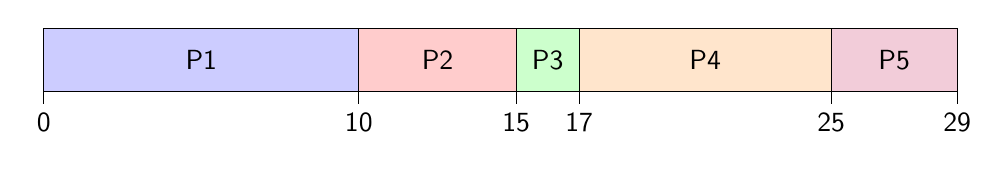
\begin{tikzpicture}[x=0.4cm, y=0.8cm, font=\sffamily]
        \draw[fill=blue!20] (0,0) rectangle (10,1) node[midway] {P1};
        \draw[fill=red!20] (10,0) rectangle (15,1) node[midway] {P2};
        \draw[fill=green!20] (15,0) rectangle (17,1) node[midway] {P3};
        \draw[fill=orange!20] (17,0) rectangle (25,1) node[midway] {P4};
        \draw[fill=purple!20] (25,0) rectangle (29,1) node[midway] {P5};
        \foreach \x in {0,10,15,17,25,29} \draw (\x,0) -- (\x,-0.2) node[below] {\x};
    \end{tikzpicture}
    }
    
    \vspace{0.4cm}
    \textbf{2. SJF (Shortest Job First - Non Preemptive)} \\
    P1 berjalan sampai selesai. Setelah itu, pilih yang terpendek dari yang sudah datang.
    \vspace{0.2cm}
    
    \resizebox{\textwidth}{!}{
    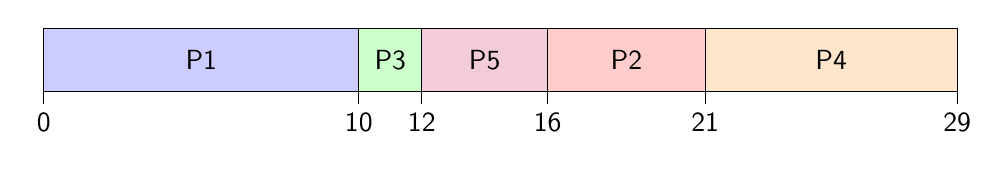
\begin{tikzpicture}[x=0.4cm, y=0.8cm, font=\sffamily]
        \draw[fill=blue!20] (0,0) rectangle (10,1) node[midway] {P1};
        \draw[fill=green!20] (10,0) rectangle (12,1) node[midway] {P3};
        \draw[fill=purple!20] (12,0) rectangle (16,1) node[midway] {P5};
        \draw[fill=red!20] (16,0) rectangle (21,1) node[midway] {P2};
        \draw[fill=orange!20] (21,0) rectangle (29,1) node[midway] {P4};
        \foreach \x in {0,10,12,16,21,29} \draw (\x,0) -- (\x,-0.2) node[below] {\x};
    \end{tikzpicture}
    }
\end{frame}

\begin{frame}
    \frametitle{Penyelesaian Soal 1: STCF \& RR}
    \footnotesize
    \textbf{3. STCF (Shortest Time-to-Completion First)} \\
    Pekerjaan baru bisa menginterupsi jika sisa waktunya lebih pendek.
    \vspace{0.1cm}
    
    \resizebox{\textwidth}{!}{
    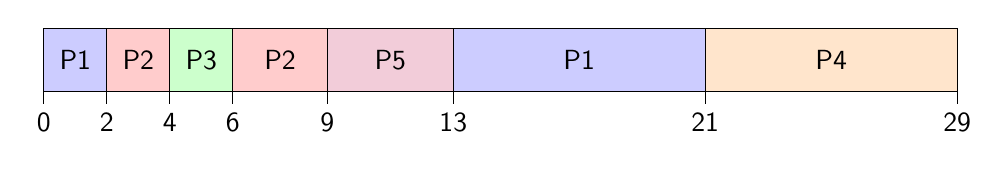
\begin{tikzpicture}[x=0.4cm, y=0.8cm, font=\sffamily]
        \draw[fill=blue!20] (0,0) rectangle (2,1) node[midway] {P1};
        \draw[fill=red!20] (2,0) rectangle (4,1) node[midway] {P2};
        \draw[fill=green!20] (4,0) rectangle (6,1) node[midway] {P3};
        \draw[fill=red!20] (6,0) rectangle (9,1) node[midway] {P2};
        \draw[fill=purple!20] (9,0) rectangle (13,1) node[midway] {P5};
        \draw[fill=blue!20] (13,0) rectangle (21,1) node[midway] {P1};
        \draw[fill=orange!20] (21,0) rectangle (29,1) node[midway] {P4};
        \foreach \x in {0,2,4,6,9,13,21,29} \draw (\x,0) -- (\x,-0.2) node[below] {\x};
    \end{tikzpicture}
    }
    
    \vspace{0.2cm}
    \textbf{4. Round Robin (q=2)} \\
    Bergantian setiap 2 ms. Adil, tapi banyak \textit{context switch}.
    \vspace{0.1cm}
    
    \resizebox{\textwidth}{!}{
    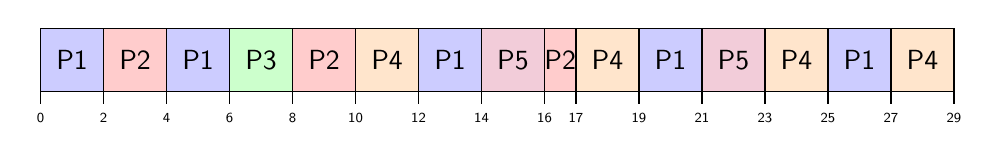
\begin{tikzpicture}[x=0.4cm, y=0.8cm, font=\sffamily]
        \draw[fill=blue!20] (0,0) rectangle (2,1) node[midway] {P1};
        \draw[fill=red!20] (2,0) rectangle (4,1) node[midway] {P2};
        \draw[fill=blue!20] (4,0) rectangle (6,1) node[midway] {P1};
        \draw[fill=green!20] (6,0) rectangle (8,1) node[midway] {P3};
        \draw[fill=red!20] (8,0) rectangle (10,1) node[midway] {P2};
        \draw[fill=orange!20] (10,0) rectangle (12,1) node[midway] {P4};
        \draw[fill=blue!20] (12,0) rectangle (14,1) node[midway] {P1};
        \draw[fill=purple!20] (14,0) rectangle (16,1) node[midway] {P5};
        \draw[fill=red!20] (16,0) rectangle (17,1) node[midway] {P2};
        \draw[fill=orange!20] (17,0) rectangle (19,1) node[midway] {P4};
        \draw[fill=blue!20] (19,0) rectangle (21,1) node[midway] {P1};
        \draw[fill=purple!20] (21,0) rectangle (23,1) node[midway] {P5};
        \draw[fill=orange!20] (23,0) rectangle (25,1) node[midway] {P4};
        \draw[fill=blue!20] (25,0) rectangle (27,1) node[midway] {P1};
        \draw[fill=orange!20] (27,0) rectangle (29,1) node[midway] {P4};
        \foreach \x in {0,2,4,6,8,10,12,14,16,17,19,21,23,25,27,29} \draw (\x,0) -- (\x,-0.2) node[below] {\tiny \x};
    \end{tikzpicture}
    }
\end{frame}

\begin{frame}
    \frametitle{Penyelesaian Soal 1: MLFQ}
    \small
    \textbf{5. MLFQ (Q3=2, Q2=4, Q1=8, Boost=20)} \\
    Pekerjaan baru masuk Q3. Jika jatah habis, turun kelas. Boost di ms ke-20.
    \vspace{0.2cm}
    
    \resizebox{\textwidth}{!}{
    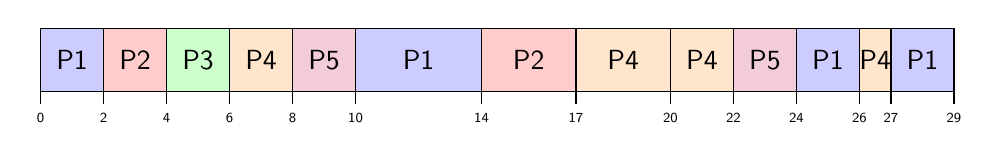
\begin{tikzpicture}[x=0.4cm, y=0.8cm, font=\sffamily]
        \draw[fill=blue!20] (0,0) rectangle (2,1) node[midway] {P1};
        \draw[fill=red!20] (2,0) rectangle (4,1) node[midway] {P2};
        \draw[fill=green!20] (4,0) rectangle (6,1) node[midway] {P3};
        \draw[fill=orange!20] (6,0) rectangle (8,1) node[midway] {P4};
        \draw[fill=purple!20] (8,0) rectangle (10,1) node[midway] {P5};
        \draw[fill=blue!20] (10,0) rectangle (14,1) node[midway] {P1};
        \draw[fill=red!20] (14,0) rectangle (17,1) node[midway] {P2};
        \draw[fill=orange!20] (17,0) rectangle (20,1) node[midway] {P4};
        \draw[fill=orange!20] (20,0) rectangle (22,1) node[midway] {P4};
        \draw[fill=purple!20] (22,0) rectangle (24,1) node[midway] {P5};
        \draw[fill=blue!20] (24,0) rectangle (26,1) node[midway] {P1};
        \draw[fill=orange!20] (26,0) rectangle (27,1) node[midway] {P4};
        \draw[fill=blue!20] (27,0) rectangle (29,1) node[midway] {P1};
        \foreach \x in {0,2,4,6,8,10,14,17,20,22,24,26,27,29} \draw (\x,0) -- (\x,-0.2) node[below] {\tiny \x};
    \end{tikzpicture}
    }
    
    \vspace{0.3cm}
    \begin{exampleblock}{Pembahasan}
        Pada MLFQ, P3 (pekerjaan terpendek) selesai sangat cepat (di ms ke-6) tanpa perlu tahu durasinya di awal. P4 sempat terpotong di ms ke-20 karena ada \textit{Priority Boost}, sehingga ia kembali ke Q3 dan langsung dieksekusi lagi.
    \end{exampleblock}
\end{frame}

\begin{frame}
    \frametitle{Analisis Metrik Soal Tantangan 1}
    \framesubtitle{Perbandingan Rata-rata RT, TAT, dan WT}
    \scriptsize
    Berdasarkan Gantt Chart sebelumnya, kita hitung rata-rata Response Time (RT), Turnaround Time (TAT), dan Waiting Time (WT) untuk 5 pekerjaan:
    \vspace{0.2cm}
    \begin{table}[]
        \centering
        \begin{tabular}{lccc}
            \toprule
            \textbf{Algoritme} & \textbf{Avg Response Time} & \textbf{Avg Turnaround Time} & \textbf{Avg Waiting Time} \\
            \midrule
            \textbf{FIFO} & 9.4 ms & 15.2 ms & 9.4 ms \\
            \textbf{SJF} & 7.8 ms & 13.6 ms & 7.8 ms \\
            \textbf{STCF} & 3.2 ms & \tem{11.6 ms} & \tem{5.8 ms} \\
            \textbf{RR (q=2)} & 2.4 ms & 16.8 ms & 11.0 ms \\
            \textbf{MLFQ} & \tem{0.0 ms} & 16.6 ms & 10.8 ms \\
            \bottomrule
        \end{tabular}
    \end{table}
    \vspace{0.2cm}
    \begin{alertblock}{Kesimpulan Soal 1}
        \begin{itemize}
            \item \textbf{Terbaik untuk Turnaround Time:} \tem{STCF}. Karena STCF selalu mendahulukan sisa pekerjaan terpendek, rata-rata waktu selesainya paling optimal.
            \item \textbf{Terbaik untuk Response Time:} \tem{MLFQ}. Karena setiap pekerjaan baru langsung diletakkan di antrean tertinggi (Q3), semua pekerjaan langsung direspons seketika (RT = 0).
        \end{itemize}
    \end{alertblock}
\end{frame}

%================================================
% PART 7: SOAL TANTANGAN 2
%================================================
\section{Soal Tantangan 2}

\begin{frame}
    \frametitle{Soal Tantangan 2: Perbandingan 5 Algoritme}
    \framesubtitle{Kasus dengan Jeda Kedatangan}
    \small
    Diberikan 5 pekerjaan dengan spesifikasi berikut:
    \begin{table}[]
        \centering
        \begin{tabular}{lcc}
            \toprule
            \textbf{Job} & \textbf{Arrival Time} & \textbf{Burst Time} \\
            \midrule
            \textbf{J1} & 0 & 12 \\
            \textbf{J2} & 3 & 4 \\
            \textbf{J3} & 5 & 6 \\
            \textbf{J4} & 9 & 2 \\
            \textbf{J5} & 12 & 5 \\
            \bottomrule
        \end{tabular}
    \end{table}
    \vspace{0.2cm}
    \textbf{Aturan:}
    \begin{itemize}
        \item \textbf{RR:} Quantum = 3
        \item \textbf{MLFQ:} Q3 (q=3), Q2 (q=5), Q1 (q=10). Boost setiap 30 ms.
    \end{itemize}
\end{frame}

\begin{frame}
    \frametitle{Penyelesaian Soal 2: FIFO \& SJF}
    \small
    \textbf{1. FIFO (First In First Out)} \\
    \vspace{0.2cm}
    
    \resizebox{\textwidth}{!}{
    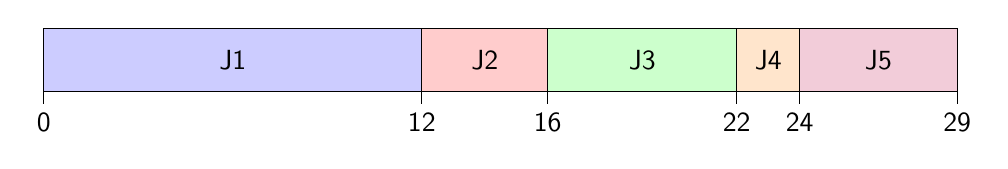
\begin{tikzpicture}[x=0.4cm, y=0.8cm, font=\sffamily]
        \draw[fill=blue!20] (0,0) rectangle (12,1) node[midway] {J1};
        \draw[fill=red!20] (12,0) rectangle (16,1) node[midway] {J2};
        \draw[fill=green!20] (16,0) rectangle (22,1) node[midway] {J3};
        \draw[fill=orange!20] (22,0) rectangle (24,1) node[midway] {J4};
        \draw[fill=purple!20] (24,0) rectangle (29,1) node[midway] {J5};
        \foreach \x in {0,12,16,22,24,29} \draw (\x,0) -- (\x,-0.2) node[below] {\x};
    \end{tikzpicture}
    }
    
    \vspace{0.4cm}
    \textbf{2. SJF (Shortest Job First - Non Preemptive)} \\
    \vspace{0.2cm}
    
    \resizebox{\textwidth}{!}{
    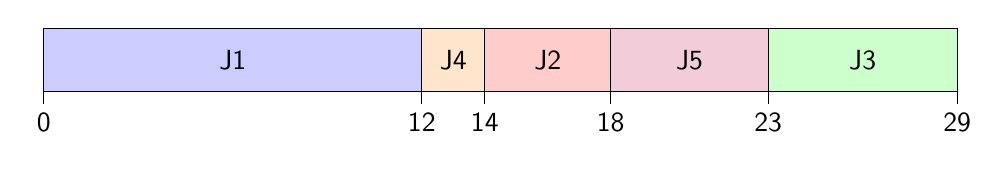
\begin{tikzpicture}[x=0.4cm, y=0.8cm, font=\sffamily]
        \draw[fill=blue!20] (0,0) rectangle (12,1) node[midway] {J1};
        \draw[fill=orange!20] (12,0) rectangle (14,1) node[midway] {J4};
        \draw[fill=red!20] (14,0) rectangle (18,1) node[midway] {J2};
        \draw[fill=purple!20] (18,0) rectangle (23,1) node[midway] {J5};
        \draw[fill=green!20] (23,0) rectangle (29,1) node[midway] {J3};
        \foreach \x in {0,12,14,18,23,29} \draw (\x,0) -- (\x,-0.2) node[below] {\x};
    \end{tikzpicture}
    }
\end{frame}

\begin{frame}
    \frametitle{Penyelesaian Soal 2: STCF \& RR}
    \footnotesize
    \textbf{3. STCF (Shortest Time-to-Completion First)} \\
    \vspace{0.1cm}
    
    \resizebox{\textwidth}{!}{
    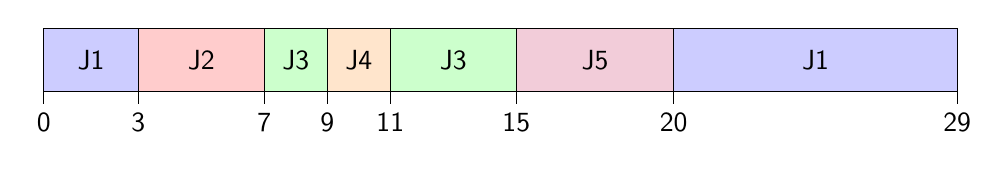
\begin{tikzpicture}[x=0.4cm, y=0.8cm, font=\sffamily]
        \draw[fill=blue!20] (0,0) rectangle (3,1) node[midway] {J1};
        \draw[fill=red!20] (3,0) rectangle (7,1) node[midway] {J2};
        \draw[fill=green!20] (7,0) rectangle (9,1) node[midway] {J3};
        \draw[fill=orange!20] (9,0) rectangle (11,1) node[midway] {J4};
        \draw[fill=green!20] (11,0) rectangle (15,1) node[midway] {J3};
        \draw[fill=purple!20] (15,0) rectangle (20,1) node[midway] {J5};
        \draw[fill=blue!20] (20,0) rectangle (29,1) node[midway] {J1};
        \foreach \x in {0,3,7,9,11,15,20,29} \draw (\x,0) -- (\x,-0.2) node[below] {\x};
    \end{tikzpicture}
    }
    
    \vspace{0.2cm}
    \textbf{4. Round Robin (q=3)} \\
    \vspace{0.1cm}
    
    \resizebox{\textwidth}{!}{
    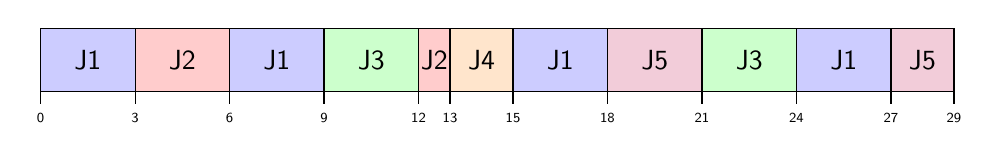
\begin{tikzpicture}[x=0.4cm, y=0.8cm, font=\sffamily]
        \draw[fill=blue!20] (0,0) rectangle (3,1) node[midway] {J1};
        \draw[fill=red!20] (3,0) rectangle (6,1) node[midway] {J2};
        \draw[fill=blue!20] (6,0) rectangle (9,1) node[midway] {J1};
        \draw[fill=green!20] (9,0) rectangle (12,1) node[midway] {J3};
        \draw[fill=red!20] (12,0) rectangle (13,1) node[midway] {J2};
        \draw[fill=orange!20] (13,0) rectangle (15,1) node[midway] {J4};
        \draw[fill=blue!20] (15,0) rectangle (18,1) node[midway] {J1};
        \draw[fill=purple!20] (18,0) rectangle (21,1) node[midway] {J5};
        \draw[fill=green!20] (21,0) rectangle (24,1) node[midway] {J3};
        \draw[fill=blue!20] (24,0) rectangle (27,1) node[midway] {J1};
        \draw[fill=purple!20] (27,0) rectangle (29,1) node[midway] {J5};
        \foreach \x in {0,3,6,9,12,13,15,18,21,24,27,29} \draw (\x,0) -- (\x,-0.2) node[below] {\tiny \x};
    \end{tikzpicture}
    }
\end{frame}

\begin{frame}
    \frametitle{Penyelesaian Soal 2: MLFQ}
    \small
    \textbf{5. MLFQ (Q3=3, Q2=5, Q1=10, Boost=30)} \\
    \vspace{0.2cm}
    
    \resizebox{\textwidth}{!}{
    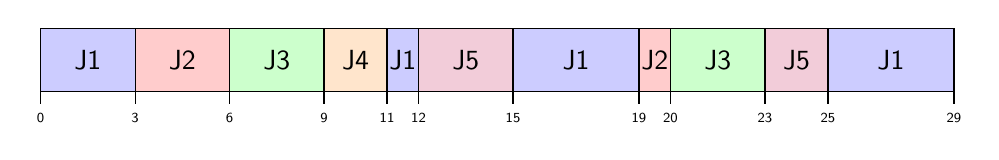
\begin{tikzpicture}[x=0.4cm, y=0.8cm, font=\sffamily]
        \draw[fill=blue!20] (0,0) rectangle (3,1) node[midway] {J1};
        \draw[fill=red!20] (3,0) rectangle (6,1) node[midway] {J2};
        \draw[fill=green!20] (6,0) rectangle (9,1) node[midway] {J3};
        \draw[fill=orange!20] (9,0) rectangle (11,1) node[midway] {J4};
        \draw[fill=blue!20] (11,0) rectangle (12,1) node[midway] {J1};
        \draw[fill=purple!20] (12,0) rectangle (15,1) node[midway] {J5};
        \draw[fill=blue!20] (15,0) rectangle (19,1) node[midway] {J1};
        \draw[fill=red!20] (19,0) rectangle (20,1) node[midway] {J2};
        \draw[fill=green!20] (20,0) rectangle (23,1) node[midway] {J3};
        \draw[fill=purple!20] (23,0) rectangle (25,1) node[midway] {J5};
        \draw[fill=blue!20] (25,0) rectangle (29,1) node[midway] {J1};
        \foreach \x in {0,3,6,9,11,12,15,19,20,23,25,29} \draw (\x,0) -- (\x,-0.2) node[below] {\tiny \x};
    \end{tikzpicture}
    }
    
    \vspace{0.3cm}
    \begin{exampleblock}{Pembahasan}
        Pada MLFQ, J1 yang panjang terus turun kelas. Saat J5 datang di ms ke-12, J5 masuk ke Q3 dan langsung menginterupsi J1 yang saat itu sedang berjalan di Q2. Ini membuktikan MLFQ sangat responsif terhadap pekerjaan baru yang interaktif.
    \end{exampleblock}
\end{frame}

\begin{frame}
    \frametitle{Analisis Metrik Soal Tantangan 2}
    \framesubtitle{Perbandingan Rata-rata RT, TAT, dan WT}
    \scriptsize
    Perhitungan rata-rata metrik untuk Soal 2 (kasus dengan jeda kedatangan):
    \vspace{0.2cm}
    \begin{table}[]
        \centering
        \begin{tabular}{lccc}
            \toprule
            \textbf{Algoritme} & \textbf{Avg Response Time} & \textbf{Avg Turnaround Time} & \textbf{Avg Waiting Time} \\
            \midrule
            \textbf{FIFO} & 9.0 ms & 14.8 ms & 9.0 ms \\
            \textbf{SJF} & 7.6 ms & 13.4 ms & 7.6 ms \\
            \textbf{STCF} & 1.0 ms & \tem{10.6 ms} & \tem{4.8 ms} \\
            \textbf{RR (q=3)} & 2.8 ms & 15.8 ms & 10.0 ms \\
            \textbf{MLFQ} & \tem{0.2 ms} & 15.8 ms & 10.0 ms \\
            \bottomrule
        \end{tabular}
    \end{table}
    \vspace{0.2cm}
    \begin{alertblock}{Kesimpulan Soal 2}
        \begin{itemize}
            \item \textbf{STCF} kembali menjadi juara mutlak untuk \tem{Turnaround Time} dan \tem{Waiting Time}.
            \item \textbf{MLFQ} sangat unggul di \tem{Response Time} (0.2 ms), hampir menyamai STCF, namun tanpa perlu mengetahui durasi pekerjaan (burst time) di awal! Inilah alasan MLFQ dipakai di OS modern.
        \end{itemize}
    \end{alertblock}
\end{frame}

%================================================
% PART 8: KESIMPULAN
%================================================
\section{Kesimpulan}

\begin{frame}
    \frametitle{Ringkasan Waktu Penyelesaian (Contoh Dasar)}
    \framesubtitle{Kapan setiap pekerjaan selesai?}
    \small
    Dari simulasi Contoh Dasar tadi, kita mendapatkan waktu selesai (Completion Time) untuk masing-masing pekerjaan:
    \vspace{0.3cm}
    \begin{table}[]
        \centering
        \begin{tabular}{lccc}
            \toprule
            \textbf{Nama Job} & \textbf{Waktu Datang} & \textbf{Burst Time} & \textbf{Waktu Selesai} \\
            \midrule
            \textbf{Job C} & 22 ms & 5 ms & \tem{30 ms} \\
            \textbf{Job B} & 15 ms & 15 ms & \tem{50 ms} \\
            \textbf{Job A} & 0 ms & 45 ms & \tem{65 ms} \\
            \bottomrule
        \end{tabular}
    \end{table}
    \vspace{0.3cm}
    \begin{alertblock}{Pelajaran Penting}
        Perhatikan bagaimana Job C (pekerjaan pendek) bisa selesai dengan cepat meskipun datang belakangan. Inilah kehebatan MLFQ: \tem{memprioritaskan pekerjaan pendek/interaktif} tanpa perlu tahu durasinya di awal!
    \end{alertblock}
\end{frame}

%================================================
% PART 9: LATIHAN MANDIRI
%================================================
\section{Latihan Mandiri}

\begin{frame}
    \frametitle{Latihan Mandiri}
    \framesubtitle{Uji Pemahaman Anda!}
    \scriptsize
    Selesaikan soal berikut menggunakan 5 algoritme (FIFO, SJF, STCF, RR, MLFQ) dan tentukan algoritme mana yang memberikan \textbf{Turnaround Time} terbaik!
    \vspace{0.2cm}
    \begin{table}[]
        \centering
        \begin{tabular}{lcc}
            \toprule
            \textbf{Job} & \textbf{Arrival Time} & \textbf{Burst Time} \\
            \midrule
            \textbf{T1} & 0 & 8 \\
            \textbf{T2} & 2 & 6 \\
            \textbf{T3} & 4 & 2 \\
            \textbf{T4} & 5 & 4 \\
            \textbf{T5} & 8 & 10 \\
            \bottomrule
        \end{tabular}
    \end{table}
    \vspace{0.2cm}
    \textbf{Aturan:}
    \begin{itemize}
        \item \textbf{RR:} Quantum = 4
        \item \textbf{MLFQ:} Q3 (q=2), Q2 (q=4), Q1 (q=8). Boost setiap 25 ms.
    \end{itemize}
\end{frame}

\begin{frame}
    \frametitle{Terima Kasih}
    \begin{center}
        \Huge \textbf{Ada Pertanyaan?}
        
        \vspace{1cm}
        \normalsize
        Jangan ragu untuk mengulang simulasi ini di atas kertas agar lebih paham!
    \end{center}
\end{frame}

\end{document}